% compile using xelatex
\documentclass{hrothgar-memo}

\usepackage[utf8]{inputenc}
\usepackage{graphicx}
\usepackage{wrapfig}

\begin{document}

%-------------------------------------------------------------------
% Memo Header
\hspace*{-10pt}
\begin{tabular}{lp{5.5in}}
    Date:    & \lowercaps{12 November 575} \abbr{CE} \\[3pt]
    To:      & Grendel \\[3pt]
    From:    & Hrothgar \\[3pt]
    Subject: & please stop it
\end{tabular} \vspace*{1em}

%-------------------------------------------------------------------
% Memo body text

\section{Introduction}
\begin{wrapfigure}{r}{0.3\textwidth}
\raggedleft
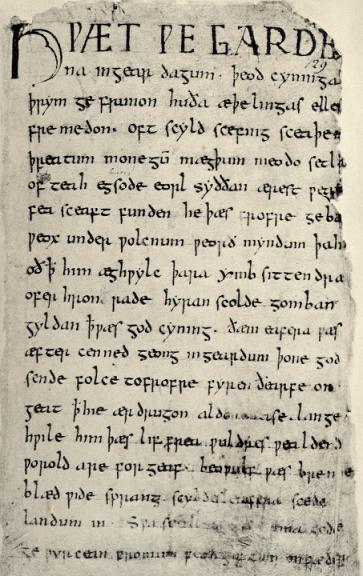
\includegraphics[width=0.28\textwidth]{beowulf.jpeg}
\end{wrapfigure}
\work{Beowulf} is the conventional title of an Old English heroic epic poem consisting of 3182 alliterative long lines, set in Scandinavia, commonly cited as one of the most important works of Anglo-Saxon literature.\footnote{All of this text was grabbed from Wikipedia on 17 \lowercaps{sep} 2013.}

\section{Manuscript}
It survives in a single manuscript known as the \work{Nowell Codex}. Its composition by an anonymous Anglo-Saxon poet is dated between the 8th and the early 11th century. In 1731, the manuscript was badly damaged by a fire that swept through a building housing a collection of Medieval manuscripts assembled by Sir Robert Bruce Cotton.

The poem's existence for its first seven centuries or so made no impression on writers and scholars, and besides a brief mention in a 1705 catalogue by Humfrey Wanley it was not studied until the end of the eighteenth century, and not published in its entirety until the 1815 edition prepared by the Icelandic-Danish scholar Gr\'imur J\'onsson Thorkelin.

\section{Story sketch}

Beowulf begins with the story of King Hrothgar, who constructed the great hall Heorot for his people. In it he, his wife Wealhtheow, and his warriors spend their time singing and celebrating, until Grendel, a troll-like monster who is pained by the noise, attacks the hall and kills and devours many of Hrothgar's warriors while they sleep. But Grendel does not touch the throne of Hrothgar, for it is described as protected by a powerful god. Hrothgar and his people, helpless against Grendel's attacks, abandon Heorot.

\begin{itemize}
\setlength{\itemsep}{1pt}
\item First battle: Grendel
\item Second battle: Grendel's mother
\item Third battle: The dragon
\end{itemize}

Beowulf is considered an epic poem in that the main character is a hero who travels great distances to prove his strength at impossible odds against supernatural demons and beasts. The poem also begins in medias res (``into the middle of affairs") or simply, ``in the middle", which is a characteristic of the epics of antiquity. Although the poem begins with Beowulf's arrival, Grendel's attacks have been an ongoing event. An elaborate history of characters and their lineages is spoken of, as well as their interactions with each other, debts owed and repaid, and deeds of valour. The warriors follow a manifest of rules on heroism called comitatus, which is the basis for all of the words, deeds, and actions.

\section{Form and metre}

An Old English poem such as Beowulf is very different from modern poetry. Anglo-Saxon poets typically used alliterative verse, a form of verse that uses alliteration as the principal structuring device to unify lines of poetry, as opposed to other devices such as rhyme, a tool which is used rather infrequently. This is a technique in which the first half of the line (the a-verse) is linked to the second half (the b-verse) through similarity in initial sound. In addition, the two halves are divided by a caesura: ``Oft Scyld Scefing / sceathena threatum" (l.~4). This is a form of accentual verse, as opposed to our accentual-syllabic verse. There are four beats in every line --- and two in every half-line.

\section{Conclusion}
In the poem, Beowulf, a hero of the Geats in Scandinavia, comes to the help of Hrothgar, the king of the Danes, whose mead hall (in Heorot) has been under attack by a monster known as Grendel. After Beowulf slays him, Grendel's mother attacks the hall and is then also defeated. Victorious, Beowulf goes home to Geatland in Sweden and later becomes king of the Geats. After a period of fifty years has passed, Beowulf defeats a dragon, but is fatally wounded in the battle. After his death, his attendants bury him in a tumulus, a burial mound, in Geatland.

J. R. R. Tolkien argued that the poem is an elegy.

%-------------------------------------------------------------------
% include a bibliography

\qedrule
\nocite{*}
\makebibsection
\bibliography{biblio}

\end{document}
